% !TeX root = Main.tex

\section{Šíření ve volném prostředí} \label{sec:evlny_volne_prostredi}
\subsection{Popis elektromagnetického pole}
Elektromagnetickým vlněním je označováno šíření nestacionárního elektromagnetického pole. Jedná se o~vektorové pole, pro jehož obecný popis je potřeba znát následující čtveřici vektorů pole v~každém bodě prostoru.\footnote{Vektory je v této práci značeny tučným písmem.}\\ 

\begin{tabular}{lll}
$\vec E$ & $[V/m]$ & intenzita elektrického pole\\
$\vec D$ & $[C/m^{2}]$ & indukce elektrická\\
$\vec B$ & $[Wb/m^{2}],[T]$ & indukce magnetická\\
$\vec H$ & $[A/m]$ & intenzita magnetického pole\\
\end{tabular}\bigskip \\
Pro řešení pole ve vakuu nebo v~prostředí se známými materiálovými konstantami postačuje jakákoliv dvojice vektorů, kdy jeden je vektorem elektrického pole a druhý magentického pole. To znamená, že libovolná dvojice z~variant $\vec E\vec B$, $\vec E\vec H$, $\vec D\vec H$ a~$\vec D\vec B$ postačuje po popis a řešení elektromagnetického pole.
Relace mezi vektory indukce a~intenzity příslušných polí popisují parametry prostředí. 

\begin{equation}
	\vec D = \varepsilon\vec E = \varepsilon_{0}\varepsilon_{r}\vec E
	\label{rce:D_epsE}
\end{equation}
\begin{equation}
	\vec B = \mu\vec H = \mu_{0}\mu_{r}\vec H
	\label{rce:B_muH}
\end{equation}
\begin{equation}
	\vec J = \sigma\vec E
	\label{rce:J_sigmaE}
\end{equation}
Rovnice \ref{rce:J_sigmaE} pro vektor proudové hustoty $\vec J$ v prostředí s volnými náboji je uvedena pro úplnost. Dále je v~tabulce \ref{tab:evlny_parametry_prostredi} popis a přehled možných materiálových parametrů prostředí včetně hodnot pro vakuum, které jsou odlišené indexem $0$. Naopak index $r$ v rovnicích (\ref{rce:D_epsE}) a (\ref{rce:B_muH}) představuje označení relativních parametrů. V závislosti na charakteru parametrů $\varepsilon$, $\mu$ a $\sigma$ se diferencuje prostředí dle několika vlastností, které jsou uvedeny v tabulce \ref{tab:evlny_vlastnosti_prostredi}.

\begin{table}[!h]
\catcode`\-=12 
\begin{center}
  	\caption{Materiálové vlastnosti prostředí}
  	\label{tab:evlny_parametry_prostredi}
\begin{tabular}{|lllp{2cm}l|}
	\hline
	permitivita		& $\varepsilon$	& [F/m] & 	& $\varepsilon_{0} = 8,854.10^{-12} $\\
	\hline
	permeabilita		& $\mu$		& [H/m] & 	& $\mu_{0} = 4\pi.10^{-7} $\\
	\hline
	měrná vodivost	& $\sigma$		& [S/m] & 	&\\
	\hline
\end{tabular}
\end{center}
\end{table}
\begin{table}[!h]
\catcode`\-=12 
\begin{center}
  	\caption{Dělení prostředí}
  	\label{tab:evlny_vlastnosti_prostredi}
\begin{tabular}{|lp{0.3cm}|l|l|}
	\hline
	{\bf Linearita}									& & {\bf lineární}	& {\bf nelineární}	\\
	závislost $\varepsilon$ $\mu$ a $\sigma$ na intenzitách pole 		& & nejsou závislé 	& závislé		\\ 
	\hline
	{\bf Homogennost}								& & {\bf homogenní}	& {\bf nehomogenní}	\\
	závislost $\varepsilon$ $\mu$ a $\sigma$ na prostorových souřadnicích 	& & nejsou závislé 	& závislé		\\
	\hline
	{\bf Izotropnost}								& & {\bf izotropní}	& {\bf anizotropní}	\\
	závislost $\varepsilon$ $\mu$ a $\sigma$ na směr vektorů intenzit pole 	& & nejsou závislé 	& závislé		\\
	\hline
\end{tabular}
\end{center}
\end{table}

V sousvislosti s existencí materiálových parametrů určitého prostředí, ve kterém se elektromagnetická vlna pohybuje se, zavádí tzv. {\bf konstanta šíření} $k=\pm \sqrt{k^{2}}$. Případně se označuje také jako {\bf vlnové číslo}. Je závislá na všech parametrech, které jsou v tabulce \ref{tab:evlny_parametry_prostredi} a navíc také na frekvenci. Vyjadřuje se tedy následovně.
\begin{displaymath}
	k=\pm \sqrt{k^{2}}=\pm\sqrt{-j\omega\mu(\sigma+j\omega\varepsilon)}\qquad [m^{-1}]
\end{displaymath}
Jde o komplexní parametr, který ovlivňuje charakter šíření elektromagnetické vlny. V literatuře se dají nalézt odlišnost v označení reálné a imaginární  části tohoto komplexního čísla. V \cite{emp} a také v zahraniční literatuře se užívá tento typ označení. 
\begin{equation}
	k = \beta - j\alpha
	\label{rce:evlny_alphabeta}
\end{equation}
\begin{description}
\item[$\beta$] [dB/m]-- se nazývá {\bf fázová konstanta}, která určuje fázi šířící se harmonické vlny
\item[$\alpha$] [rad/m] -- je označován {\bf měrný útlum}, vyjadřující změnu amlituda vlny
\end{description}

Podle \cite[str. 33]{emp} existují dva možné přístupy k~řešení polí, související s~časovou proměnností pole. Tato práce se zabývá odvození rovnice a řešení elektromagentického pole nestacionárního.
\begin{description}
\item[Stacionární pole]Určují se všechny zdroje a následně ke každému z~nich jejich prostorové rozložení pole. Výsledkem je superpozice všech polí.
\item[Nestacionární pole]Sestavíme diferenciální rovnici pro některý z~vektorů pole. Následně nalezneme obecné řešení a dle okrajových podmínek vybereme nejvhodnější. 
\end{description}


\subsubsection*{Obecná vlnové rovnice diferenciálního charakteru.}
 Podrobné odvození vlnových rovnic pro vektory pole $\vec E$ a $\vec B$, pro časově neměnné parametry prostředí, se nachází v~příloze \ref{sec:Odvozeni_CasPole}.
\begin{equation}
	\nabla^{2}\vec E -\mu\sigma\frac{\partial\vec E}{\partial t}-\mu\varepsilon\frac{\partial^{2}\vec E}{\partial t^{2}} = \grad\frac{\rho}{\varepsilon}+\mu\frac{\partial\vec J_{vn}}{\partial t}
	\label{rce:evlny_VlnR_ElPole}
\end{equation}
\begin{equation}
	\nabla^{2}\vec B -\mu\sigma\frac{\partial\vec B}{\partial t}-\mu\varepsilon\frac{\partial^{2}\vec B}{\partial t^{2}}= -\mu\rot\vec J_{vn}
	\label{rce:evlny_VlnR_MagPole}
\end{equation}

\subsection{Harmonické pole}
Vztahy (\ref{rce:evlny_VlnR_ElPole}) a (\ref{rce:evlny_VlnR_MagPole}), eventuelně vztahy uvedené v příloze \ref{sec:Odvozeni_CasPole}, jsou platné pro obecnou časovo závislost zdrojových funkcí $\rho$ a $\vec J_{vn}$. Pro řešení polí, především numerického charakteru, se využívají harmonické funkce ($sin$ nebo $cos$). Důvodem je komplikované až nemožné analytické řešení rovnic (\ref{rce:VlnR_ElPole}) a (\ref{rce:VlnR_MagPole}). Dále proto, že harmonické pole je možné snadno generovat a řada zařízení je založena na jejich využití. 

Pro časově proměnné harmonické pole je možné využít tzv. symbolicko - komplexní metodu. Její aplikace spočívá ve vyjádření daného vektoru pole pomocí fázoru vektoru. Ten totiž je závislý jen na postorových souřadnicích a není časově proměnný.

Pokud se bude například intenzita elektrického pole elektrického pole $\vec E(x,y,z,t)$ měnit harmonicky v~závislosti na čase, můžeme jí zapsat takto.
\begin{displaymath}
	\vec E(x,y,z,t) = \vec E(x,y,z)sin\omega t
\end{displaymath}
V daném poli je možné vyjádřit vektror intenzity elektrického pole právě pomocí fázoru vektoru $\vec E(x,y,z)$. Z něj je možné vytvořit rotující fázor vektoru.
\begin{equation}
	\dot{\vec E}(x,y,z) = \vec E(x,y,z)e^{j\omega t}
	\label{rce:rotujici_fazor_vektoru}
\end{equation}
Nakonec lze určit časovou závislost vektoru pole pomocí vztahu.
\begin{equation}
	\vec E(x,y,z,t) = Im\Big\{ \dot{\vec E}(x,y,z)\Big\} = Im\Big\{ \vec E(x,y,z)e^{j\omega t}\Big\}
	\label{rce:casova_zavislost}
\end{equation}
Z rovnice (\ref{rce:casova_zavislost}) vyplývají pro reprezentaci časově proměnného vektoru pole $\vec E(x,y,z,t)$ fázorem $\vec E(x,y,z)$ následující vlastnosti pro obraz derivace a integrálu fázoru. Ty jsou využity při odvození vlnových rovnic v harmonickém prostředí v příloze \ref{sec:Odvozeni_HarmPole}.
\begin{displaymath}
	\frac{\partial \vec E(x,y,z,t)}{\partial t} \longrightarrow j\omega \vec E(x,y,z)
\end{displaymath}
\begin{displaymath}
	\frac{\partial^{n} \vec E(x,y,z,t)}{\partial t^{n}} \longrightarrow (j\omega)^{n} \vec E(x,y,z)
\end{displaymath}
\begin{displaymath}
	\int\!\!\vec E(x,y,z,t) dt \longrightarrow \frac{\vec E(x,y,z)}{j\omega}
\end{displaymath}
\begin{displaymath}
	\int\underbrace{\ldots}_{n}\int\!\!\vec E(x,y,z,t) dt \longrightarrow \frac{\vec E(x,y,z)}{(j\omega)^{n}}
\end{displaymath}

\subsubsection*{Vlnové rovnice harmonického pole.}
 Podrobné odvození vlnových rovnic harmonického pole pro vektory $\vec E$ a $\vec B$, pro konstantní parametry $\varepsilon$, $\mu$ a $\sigma$, se nachází v~příloze \ref{sec:Odvozeni_HarmPole}.
\begin{equation}
	\nabla^{2}\vec E +k^{2}\vec E = \grad\frac{\rho}{\varepsilon}+ j\omega\mu\vec J_{vn}
	\label{rce:evlny_VlnR_ElPole_harm} 
\end{equation}
\begin{equation}
	\nabla^{2}\vec B +k^{2}\vec B = -\mu\rot\vec J_{vn}
	\label{rce:evlny_VlnR_MagPole_harm} 
\end{equation}

\subsection{Rovinná homogenní vlna ve volném prostředí}
Princip šíření elektromagnetických vln ve volném prostředí lze z několika důvodů demonstrovat na jednoduché variantě rovinné homogenní vlny, ačkoliv se vlny v této formě téměř nevyskytují. Je to dáno především omezeností rozměrů zdroje elektromagnetického záření. Avšak pro dostatečnou vzdálenost od tohoto reálného zdroje lze podle obrázku \ref{obr:evlny_rovinna_vlna} aplikovat zjednodušení, při kterém se část sférické vlnopolochy ve volném prostředí považuje za rovinnou. Pro užití rovinných homogenních vln svědčí také nezanedbatelný fakt, že pomocí jejich součtu je možné sestavit libovolnou složitější obecnou vlnu. 

\begin{figure}[!h]
	\centering
	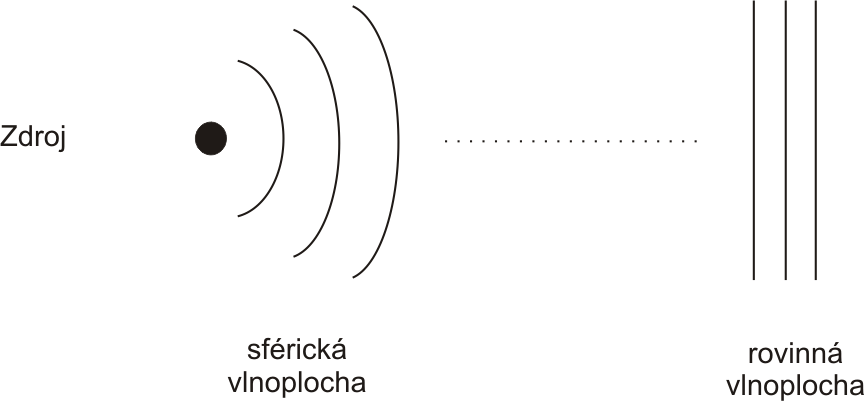
\includegraphics[width=9cm]{evlny_rovinna_vlna.png}
	\caption{Přiblížení rovinné vlny ve vzdáleném prostředí.}
	\label{obr:evlny_rovinna_vlna}
\end{figure}

V teorii šíření elektromagnetických vln se dle \cite{emp} užívá řada pojmů, z nichž některé jsou použity také v~této práci.
\begin{description}
\item[Vlnoplocha] Skupina bodů, které mají stejnou fázi a po jejich spojení tvoří geometrickou plochu vlny.
\item[Volné neohraničené prostředí] Prostor bez jakýkoliv překážek, kterými jsou předměty nebo objekty s odlišnými materiálovými konstatami  $\varepsilon$, $\mu$ a $\sigma$ od prostředí, ve kterém se vlna šíří.
\item[Homogenní vlna] Označuje se také jako {\bf uniformní} a jedná se o vlnu, která má na dané vlnoploše také konstatní amplitudu.
\end{description}

Pro analýzu libovolného obecného typu vln je nejprve potřeba zvolit vhodnou souřadnou soustavu. V případě rovinné vlny se bude jednat o kartézskou souřadnou soustavu. V harmonickém poli bez vnějších zdrojů bude odvození vycházet z homogenní Helmholtzovy rovnice (\ref{rce:VlnR_ElPole_harm_BezZdroju})
\begin{equation}
	\nabla^{2}\vec E +k^{2}\vec E = 0
	\label{rce:evlny_VlnR_ElPole_harm_BezZdroju}
\end{equation}
Aplikací Laplaceova operátoru $\nabla^{2}$ na vektor $\vec E$ dostaneme opět vektoru, který lze v kartézské soustavě vyjádřit $\nabla^{2}\vec E = \nabla^{2} E_{x}\vec x_{0} + \nabla^{2} E_{y}\vec y_{0} + \nabla^{2} E_{z}\vec z_{0}$. To způsobí rozpad vektorové rovnice (\ref{rce:evlny_VlnR_ElPole_harm_BezZdroju}) na tři podobné skalární rovnice.
\begin{displaymath}
	\nabla^{2} E_{x} +k^{2} E_{x} = 0
\end{displaymath}
\begin{displaymath}
	\nabla^{2} E_{y} +k^{2} E_{y} = 0
\end{displaymath}
\begin{displaymath}
	\nabla^{2} E_{z} +k^{2} E_{z} = 0
\end{displaymath}
Řešení této soustavy rovnic je možné provést {\bf metodou separace proměnných} nebo po zavedení určitých zjednodušujících podmínek jako {\bf jednorozměrnou diferenciální rovnici}, jak je naznačeno dále. Pro vysvětlení druhé varianty se nejprve tyto skalární vztahy rozepíšou následujícím způsobem.
\begin{equation}
	\frac{\partial ^{2} E_{x}}{\partial x^{2}} + \frac{\partial ^{2} E_{x}}{\partial y^{2}} + \frac{\partial ^{2} E_{x}}{\partial z^{2}} + k^{2} E_{x} = 0
	\label{rce:evlny_skalarni1}
\end{equation}
\begin{equation}
	\frac{\partial ^{2} E_{y}}{\partial x^{2}} + \frac{\partial ^{2} E_{y}}{\partial y^{2}} + \frac{\partial ^{2} E_{y}}{\partial z^{2}} + k^{2} E_{y} = 0
	\label{rce:evlny_skalarni2}
\end{equation}
\begin{equation}
	\frac{\partial ^{2} E_{z}}{\partial x^{2}} + \frac{\partial ^{2} E_{z}}{\partial y^{2}} + \frac{\partial ^{2} E_{z}}{\partial z^{2}} + k^{2} E_{z} = 0
	\label{rce:evlny_skalarni3}	
\end{equation}
Je vhodné zvolit souřadnou soustavu tak, aby se vlna šířila ve směru jedné z os. Poté bude platit, že vlnoplocha je rovina kolmá na tuto osu, tak jak je naznačeno na obrázku \ref{obr:evlny_vlnoplocha}. Současně uvažujeme pro zjednodušení vektor intenzity elektrického pole $\vec E$ pouze ve směru osy $x$. Je možné jej také vyjádřit jako $\vec E = E_{x}\vec {x_{0}}$.

\begin{figure}[!h]
	\centering
	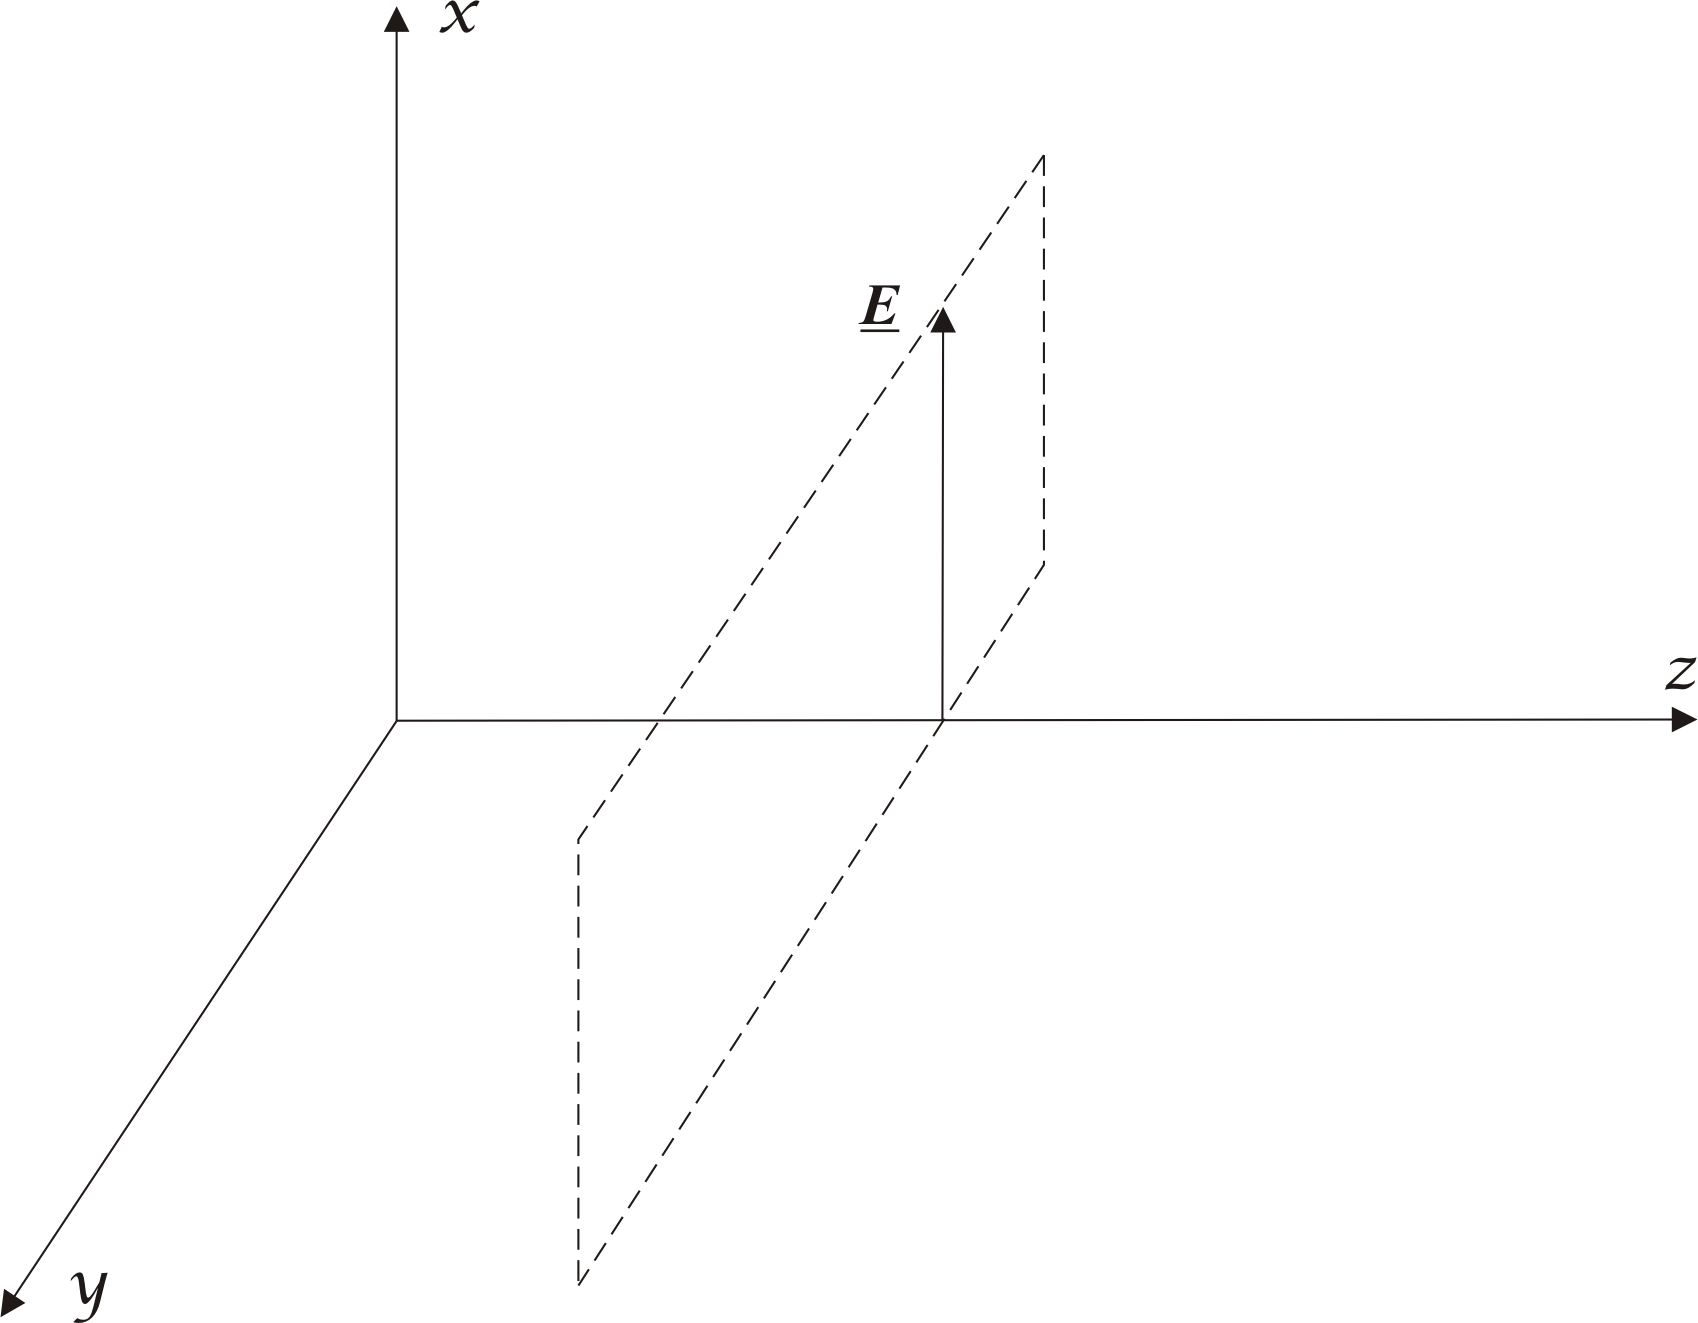
\includegraphics[width=10cm]{evlny_vlnoplocha.png}
	\caption{Vlnoplocha rovinné homogenní vlny. \cite{emp}}
	\label{obr:evlny_vlnoplocha}
\end{figure}

Z výše uvedených úvah o charakteru vln a jejich prostorového uspořádání vyplývají následující skutečnosti.
\begin{itemize*}
\item konstantní velikost a fáze vektoru $\vec E$ ve směru $x$, tzn. $\frac{\partial  E_{x}}{\partial x}=0$ a $\frac{\partial  E_{x}}{\partial y}=0$
\item nulový vektor $\vec E$ ve směru $y$, tzn. $ E_{y} = 0$
\item nulový vektor $\vec E$ ve směru $z$, tzn. $ E_{z} = 0$
\end{itemize*}
Pokud je aplikujeme na tři rozepsané skalární rovnice (\ref{rce:evlny_skalarni1}) až (\ref{rce:evlny_skalarni3}), dojde ke značnému matematickému zjenodušení. Rovnice (\ref{rce:evlny_skalarni2}) a (\ref{rce:evlny_skalarni3}) se úplně eliminují, u rovnice (\ref{rce:evlny_skalarni1}) vypadnou první dva členy. Výsledná rovnice bude tak jednorozměrná obyčejná diferenciální druhého řádu.
\begin{equation}
	\frac{\partial ^{2} E_{x}}{\partial z^{2}} + k^{2} E_{x} = 0
	\label{rce:evlny_skalarni}	
\end{equation}

\subsubsection*{Řešení rovnice rovinné homohenní vlny (\ref{rce:evlny_skalarni})}
Vzhledem k jednoduchosti dané diferenciální rovnice můžeme rovnou předpokládat řešení v následujícím tvaru, který představuje superpozici dvou funkcí.
\begin{equation}
	E_{x}(z) = E_{0}^{+}e^{\lambda_{1}z} +E_{0}^{-}e^{\lambda_{2}z}
	\label{rce:evlny_reseni1}	
\end{equation}
Výrazy $E_{0}^{+}$ a $E_{0}^{-}$ jsou komplexní konstanty dané složky vektoru. Parametry $\lambda_{1}$ a $\lambda_{2}$ se určují jako kořeny charakteristického polynomu dané diferenciální rovnice (\ref{rce:evlny_skalarni}). 
\begin{displaymath}
	\lambda^{2} + k^{2}= 0
\end{displaymath}
\begin{displaymath}
	\lambda_{1,2} = \pm \sqrt{-k^{2}}
\end{displaymath}
\begin{displaymath}
	\lambda_{1} = -jk
\end{displaymath}
\begin{displaymath}
	\lambda_{2} = +jk
\end{displaymath}
Dosazením do (\ref{rce:evlny_reseni1}) dostaneme vztah, který má jednoduché fyzikální vysvětlení. Podle obrázku \ref{obr:evlny_vlnoplocha} je zřejmé, že řešení vlnové rovnice je závislé pouze na souřadnici $z$ a vlnoplocha leží v rovice $xy$. Takto vyjádřená vlna má pouze jeden stupeň volnosti a může se tedy šířit pouze v kladném nebo záporném ve směru $z$.
\begin{equation}
	E_{x}(z) = E_{0}^{+}e^{-jkz} + E_{0}^{-}e^{jkz}
	\label{rce:evlny_reseni2}	
\end{equation}
První člen $ E_{0}^{+}e^{-jkz}$ přestavuje funkci vlny šířící se v kladném směru osy $z$ a označuje se jako {\bf postupná vlna}. Druhý člen $E_{0}^{-}e^{jkz}$ popisuje funkci vlny pohybující se v opačném směru, tzn. {\bf vlna odražená}.

Komplexní konstanty $E_{0}^{+}$ a $E_{0}^{-}$ je možné dále blíže rozepsat na část představující modul a část pro reprezentaci fázi.
\begin{displaymath}
	E_{0}^{\pm} = E_{0mod}^{\pm}e^{j\varphi_{\pm}}
\end{displaymath}
S využitím této vlastnosti upravíme rovnici (\ref{rce:evlny_reseni2}). Současně aplikujeme vztah konstanty šíření (\ref{rce:evlny_alphabeta}), tj. $k = \beta - j\alpha$.
\begin{displaymath}
	E_{x}(z) = E_{0mod}^{+}e^{j\varphi_{+}}e^{-j(\beta - j\alpha)z} + E_{0mod}^{-}e^{j\varphi_{-}}e^{j(\beta-j\alpha)z}
\end{displaymath}
Pro určení časové závislosti se nejprve užije vztah (\ref{rce:rotujici_fazor_vektoru}).
\begin{displaymath}
	\dot{E}_{x}(z) = E_{0mod}^{+}e^{j\varphi_{+}}e^{-j\beta z}e^{-\alpha z}e^{j\omega t} + E_{0mod}^{-}e^{j\varphi_{-}}e^{j\beta z}e^{\alpha z}e^{j\omega t}
\end{displaymath}
Nakonec se dle (\ref{rce:casova_zavislost}) vyjádří okamžitá hodnota časově proměnné intenzity elektrického pole. Výsledný vztah reprezentuje okamžitou hodnotu postupné a odražené složky rovinné vlny v harmonickém prostředí.
\begin{equation}
	E_{x}(z,t) = E_{0mod}^{+}e^{-\alpha z}sin(\omega t - \beta z + \varphi_{+}) + E_{0mod}^{-}e^{\alpha z}sin(\omega t + \beta z + \varphi_{-})
	\label{rce:evlny_postupna_odrazena}
\end{equation}

\begin{figure}[!h]
	\centering
	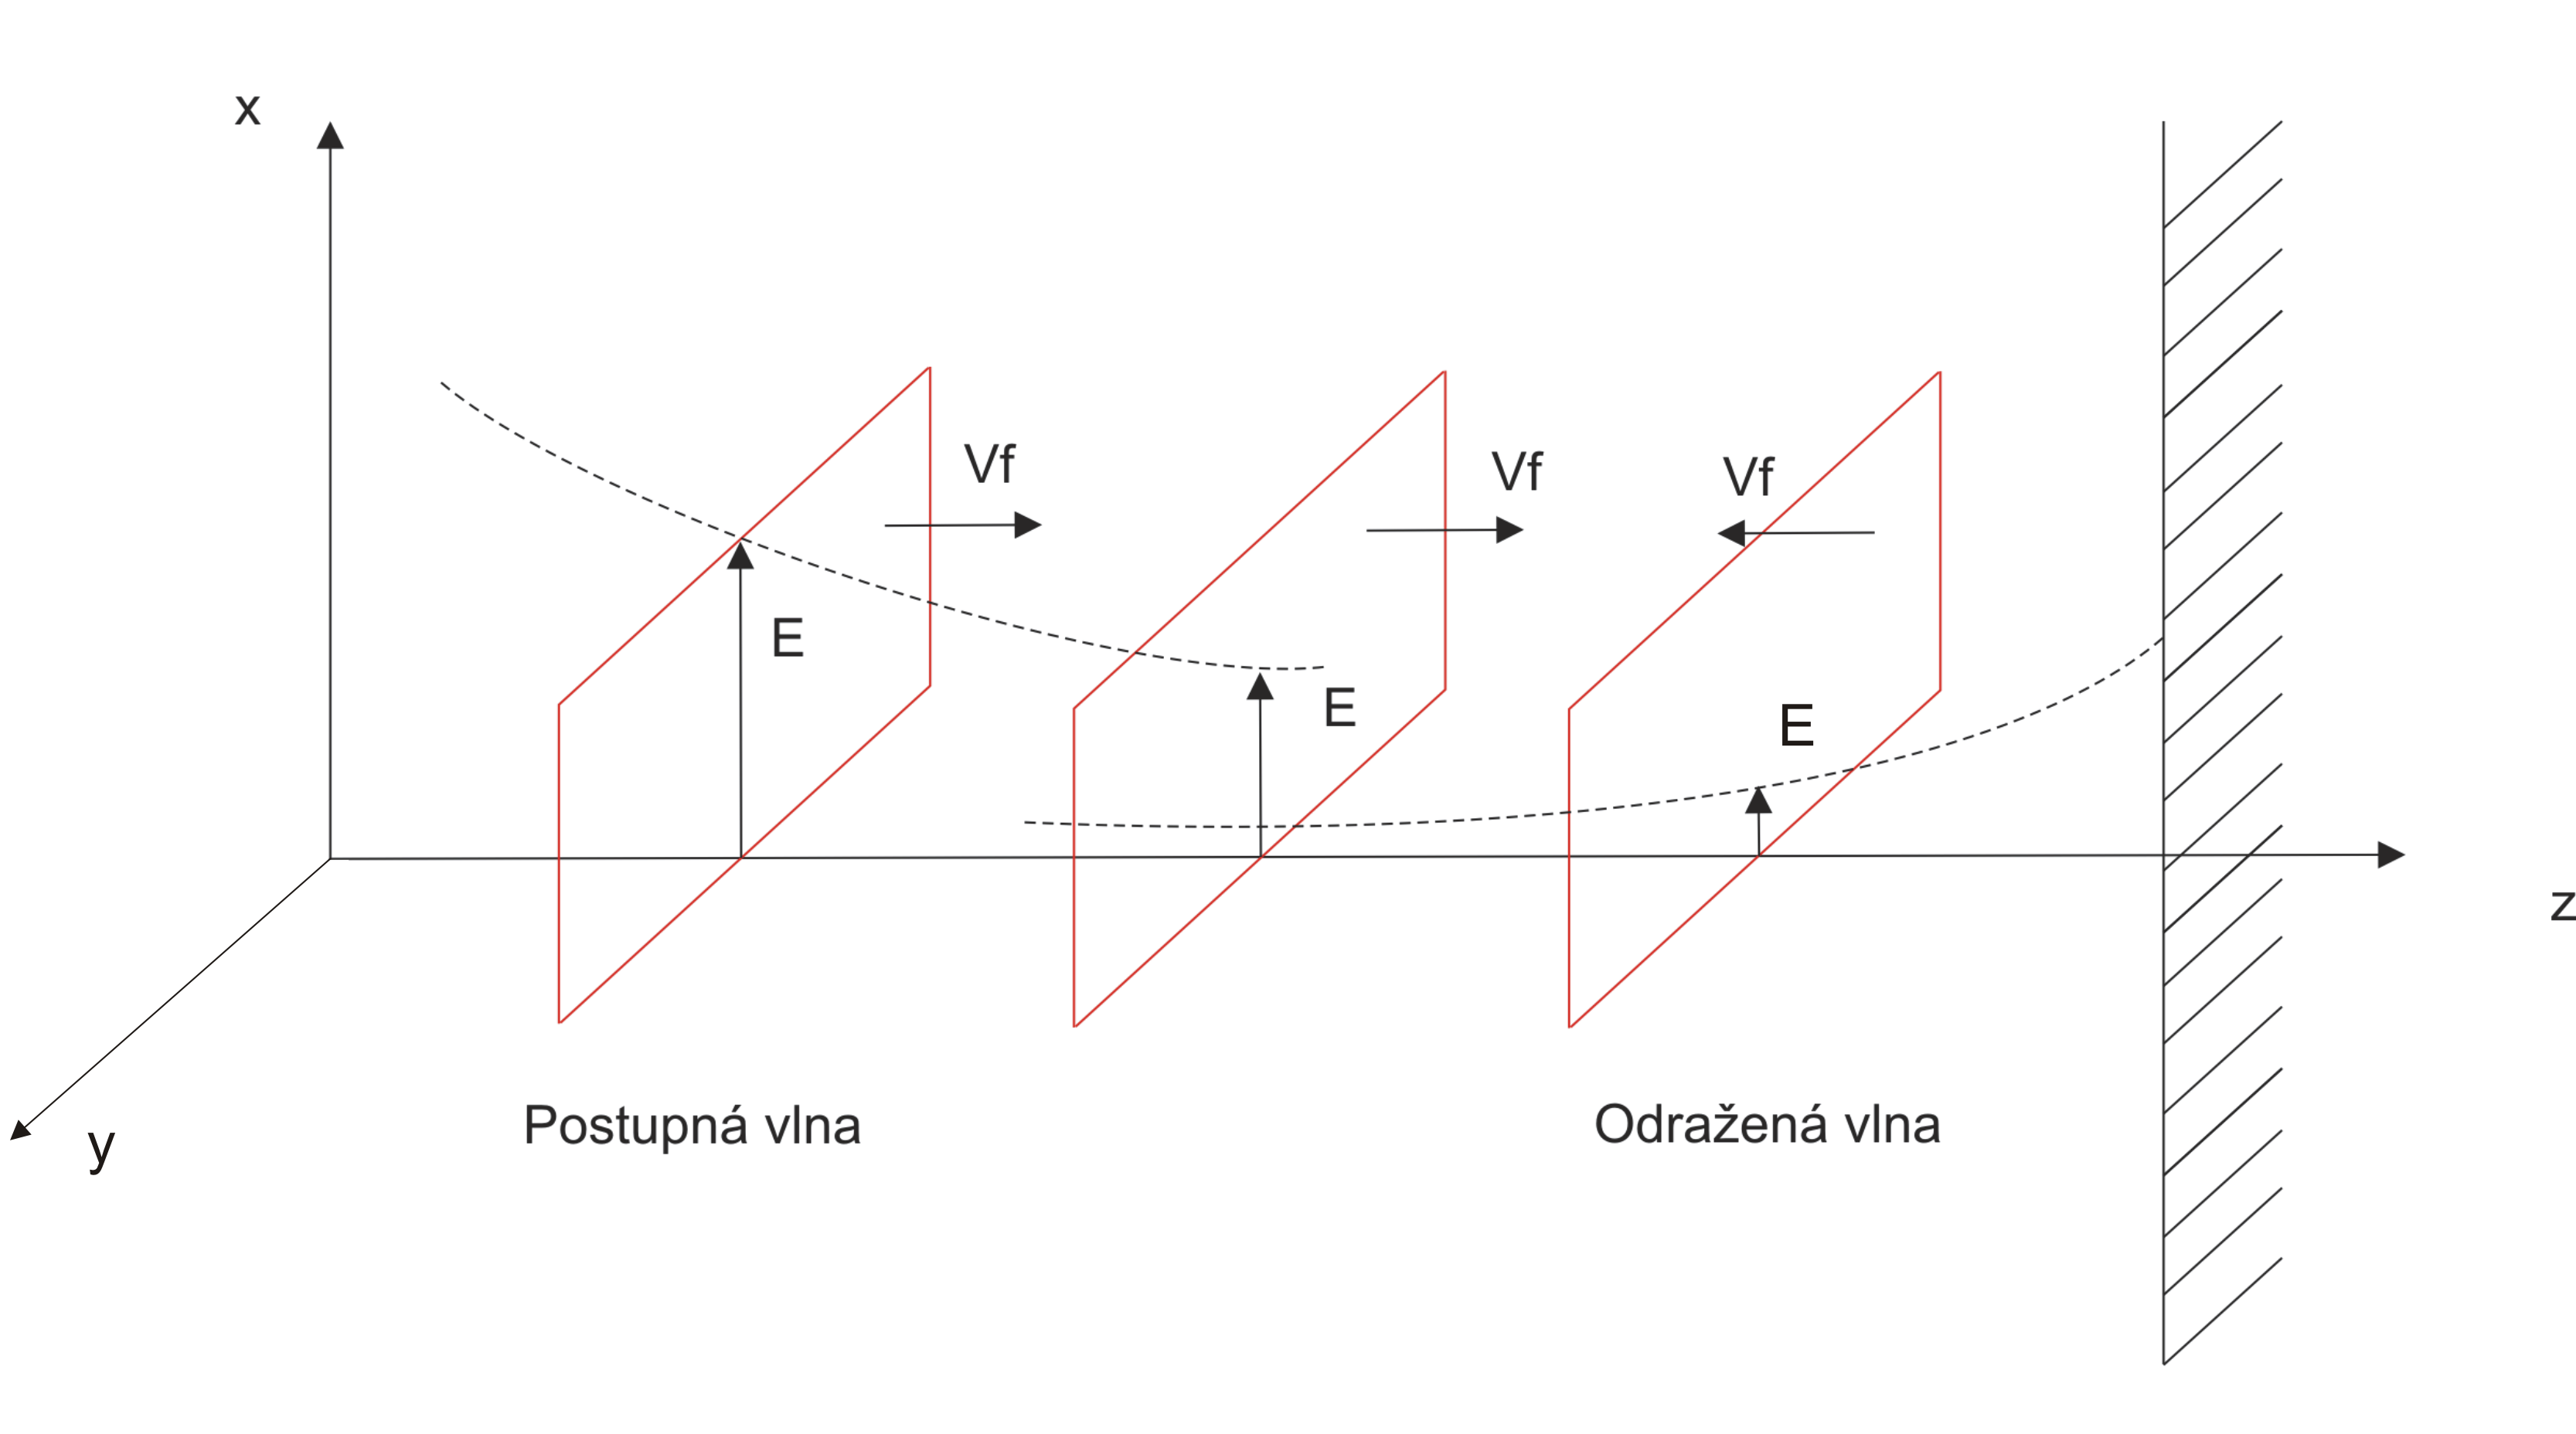
\includegraphics[width=14cm]{evlny_postupna_odrazena.png}
	\caption{Šíření postupné a odražené rovinné homogenní vlny dle (\ref{rce:evlny_postupna_odrazena}).}
	\label{obr:evlny_postupna_odrazena}
\end{figure}
\subsubsection*{Fázová rychlost vlny $v_{f}$}
Na obrázku \ref{obr:evlny_postupna_odrazena} je naznačen směr pohybu vln pomocí $v_{f}$. Rychlost, kterou se vlnoplocha ve směru osy $z$ pohybuje se označuje jako {\bf fázová rychlost vlny}. Výraz pro vyjádření odvodíme z rovnice (\ref{rce:evlny_postupna_odrazena}). Vzhledem k tomu, že vlnoplocha představuje rovinu bodů se stejnou fází, bude v rovnici platit, $\omega t - \beta z + \varphi_{+} = konst.$ pro postupnou a $\omega t + \beta z + \varphi_{-} = konst.$ pro odraženou vlnu.

Pro odvození fázové rychlosti postupné vlny zderivujeme výraz $\omega t - \beta z + \varphi_{+} = konst.$ podle času a následně upravíme.
\begin{displaymath}
	\omega - \beta \frac{dz}{dt} = 0
\end{displaymath}
\begin{displaymath}
	v_{f} = \frac{dz}{dt} = \frac{\omega}{\beta}  \ \ \ [m/s]
\end{displaymath}
Analogickým odvození z výrazu pro odraženou vlnu  $\omega t + \beta z + \varphi_{-} = konst.$ dostaneme vztah, který potvrzuje skutečnost, že odražená vlna se šíří podle osy $z$ v opačném směru 
\begin{displaymath}
	v_{f} = - \frac{\omega}{\beta}  \ \ \ [m/s]
\end{displaymath}

\subsubsection*{Obecné řešení rovnice (\ref{rce:evlny_VlnR_ElPole_harm_BezZdroju}) metodou separace proměnných}
V řadě aplikacích není možné zavédst pro řešení rovnice $\nabla^{2}\vec E +k^{2}\vec E = 0$  zjednodušující předpoklady, vycházející z obrázku \ref{obr:evlny_vlnoplocha}. Potom se rovnice řeší obecněji pomocí metody separace proměnných. Principem je nalézt řešení pro jednotlivé složky vektoru $\vec E$ pomocí součinu tří funkcí, vždy jedné proměnné, tak jak je naznačeno níže.
\begin{equation}
	E_{i}(x,y,z) = X(x).Y(y).Z(z)\qquad i = x, y, z
	\label{rce:evlny_obecne_xyz}
\end{equation}
Podrobné odvození je rozepsáno v \cite[str. 50]{emp}. Řešení je ve tvaru součinů jako (\ref{rce:evlny_obecne_xyz}).
\begin{equation}
	E_{i}(x,y,z) = \big( C_{1}e^{jk_{x}x} + C_{2}e^{-jk_{x}x} \big)\big( C_{3}e^{jk_{y}y} + C_{4}e^{-jk_{y}y} \big)\big( C_{5}e^{jk_{z}z} + C_{6}e^{-jk_{z}z} \big)
	\label{rce:evlny_obecne_reseni}
\end{equation}
Všechny neznámé konstanty se určují na základě okrajových podmínek. Komplexní konstanty $C_{1,\ldots,6}$ udávají amlitudu a fázi rovinných vln, složky konstanty šíření $k_{x}$, $k_{y}$ a $k_{z}$ určují směry šíření. Pomocí součtu určitého množství rovinných vln je tedy možné sestavit v kartézské souřadné soustavě libovolnou vlnu.

\section{Rozhraní dvou prostředí}
Podkapitola \ref{sec:evlny_volne_prostredi} se věnuje šíření elektromagnetických vln ve volném neohraničeném prostředí. Avšak pro reálnější popis je potřeba uvažovat také vliv překážek v prostorově omezené oblasti. Důležitým stavebním kamenem pro formulování tohoto problém je, jak napovídá název podkapitoly, chování vln na rozhraní mezi odlišnými prostředími.

Při dopadu elektromagnetické vlny na materiálově odlišný objekt může dojít k několika událostem, kterými jsou odraz, lom nebo prostup vlny. V praxi se přirozeně nejedná striktně o jeden typ chování. Častěji dojde k jejich kombinaci, ve které mají jednotlivé složky určité zastoupení. Fyzikální vysvětlení spočívá v existenci vodivých a posuvných proudů, které vzniknou právě při dopadu elektromagnetické vlny. Proudy představují zdroje pro vznik dalších vln, které se superponují k původní vlně a ovlivní její vlastnosti. 

Matematický popis je možný u některých příkladů po zavedení určitých zjednodušujících předpokladů. Vytvoření modelu pro obecný reálný případ nemusí být mnohdy vůbec proveditelné, neboť po dopadu vlny na překážku mohou nastat velmi komplikované procesy. Pro názornost je níže vysvětleno o jaké procesy se může jednat v jednoduchém případě rovinné homogenní vlny dopadající na rovinné rozhraní.

\subsection*{Chování rovinné vlny na rovinném rozhraní}
Tento případ by se z hlediska matematického popisu dal nazvat jako téměř ideální. V reálných variantách bude situace přirozeně jiná, ale i na tomto jednoduchém příkladu je možné popsat jevy, které nastanou po dopadu elektromagnetické vlny. 

Po popis šíření se výhodně využívá tzv. vlnový vektor $\vec k$. S jeho pomocí lze snadno názorně popsat směry šíření vln na rozhraní. Vlnový vektor představuje to, v jakém směru se šíří vlnoplocha. Dle obrázku \ref{obr:evlny_vlnovy_vektor} jej lze definovat.

\begin{displaymath}
	\vec k = k \vec{n_{0}} = k_{x}\vec{x_{0}} +  k_{y}\vec{y_{0}} +  k_{z}\vec{z_{0}}
\end{displaymath}

\begin{figure}[!h]
	\centering
	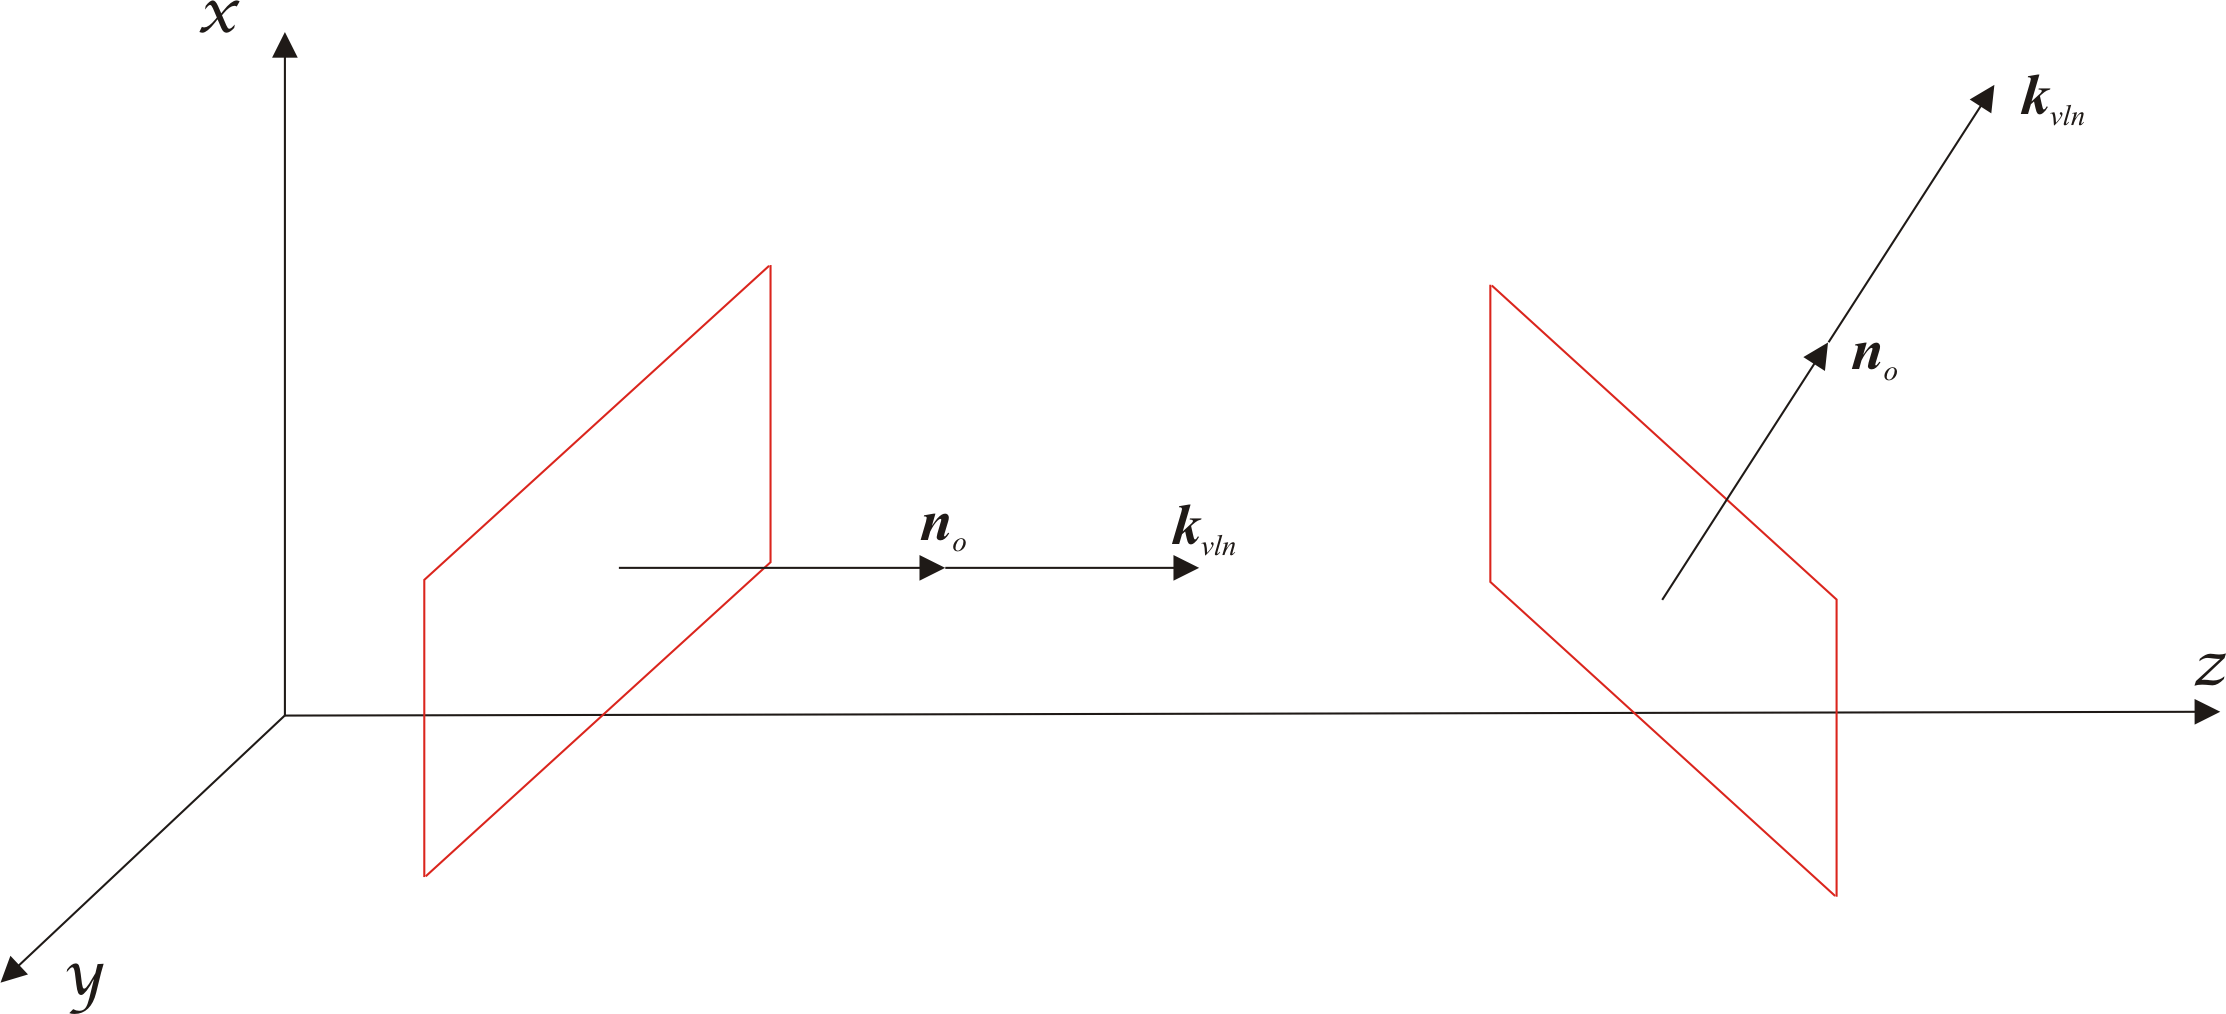
\includegraphics[width=12cm]{evlny_vlnovy_vektor.png}
	\caption{Definice vlnového vektoru v kartézské soustavě souřadnic.\cite{emp}}
	\label{obr:evlny_vlnovy_vektor}
\end{figure}

Podle naznačené situace na obrázku \ref{obr:evlny_rovinne_rozhrani} je zřejmé, jak se může zachovat elektromagnetická vlna při dopadu pod obecným úhlem na rovinné rozhraní. Může dojít k odrazu od rozhraní nebo průchodu do sousedícího prostředí, přičemž se se změní směr šíření (dojde k lomu). Nejčastější bude případ, kdy se část vlny odrazí a současně část projde a bude se lámat. 

\begin{figure}[!h]
	\centering
	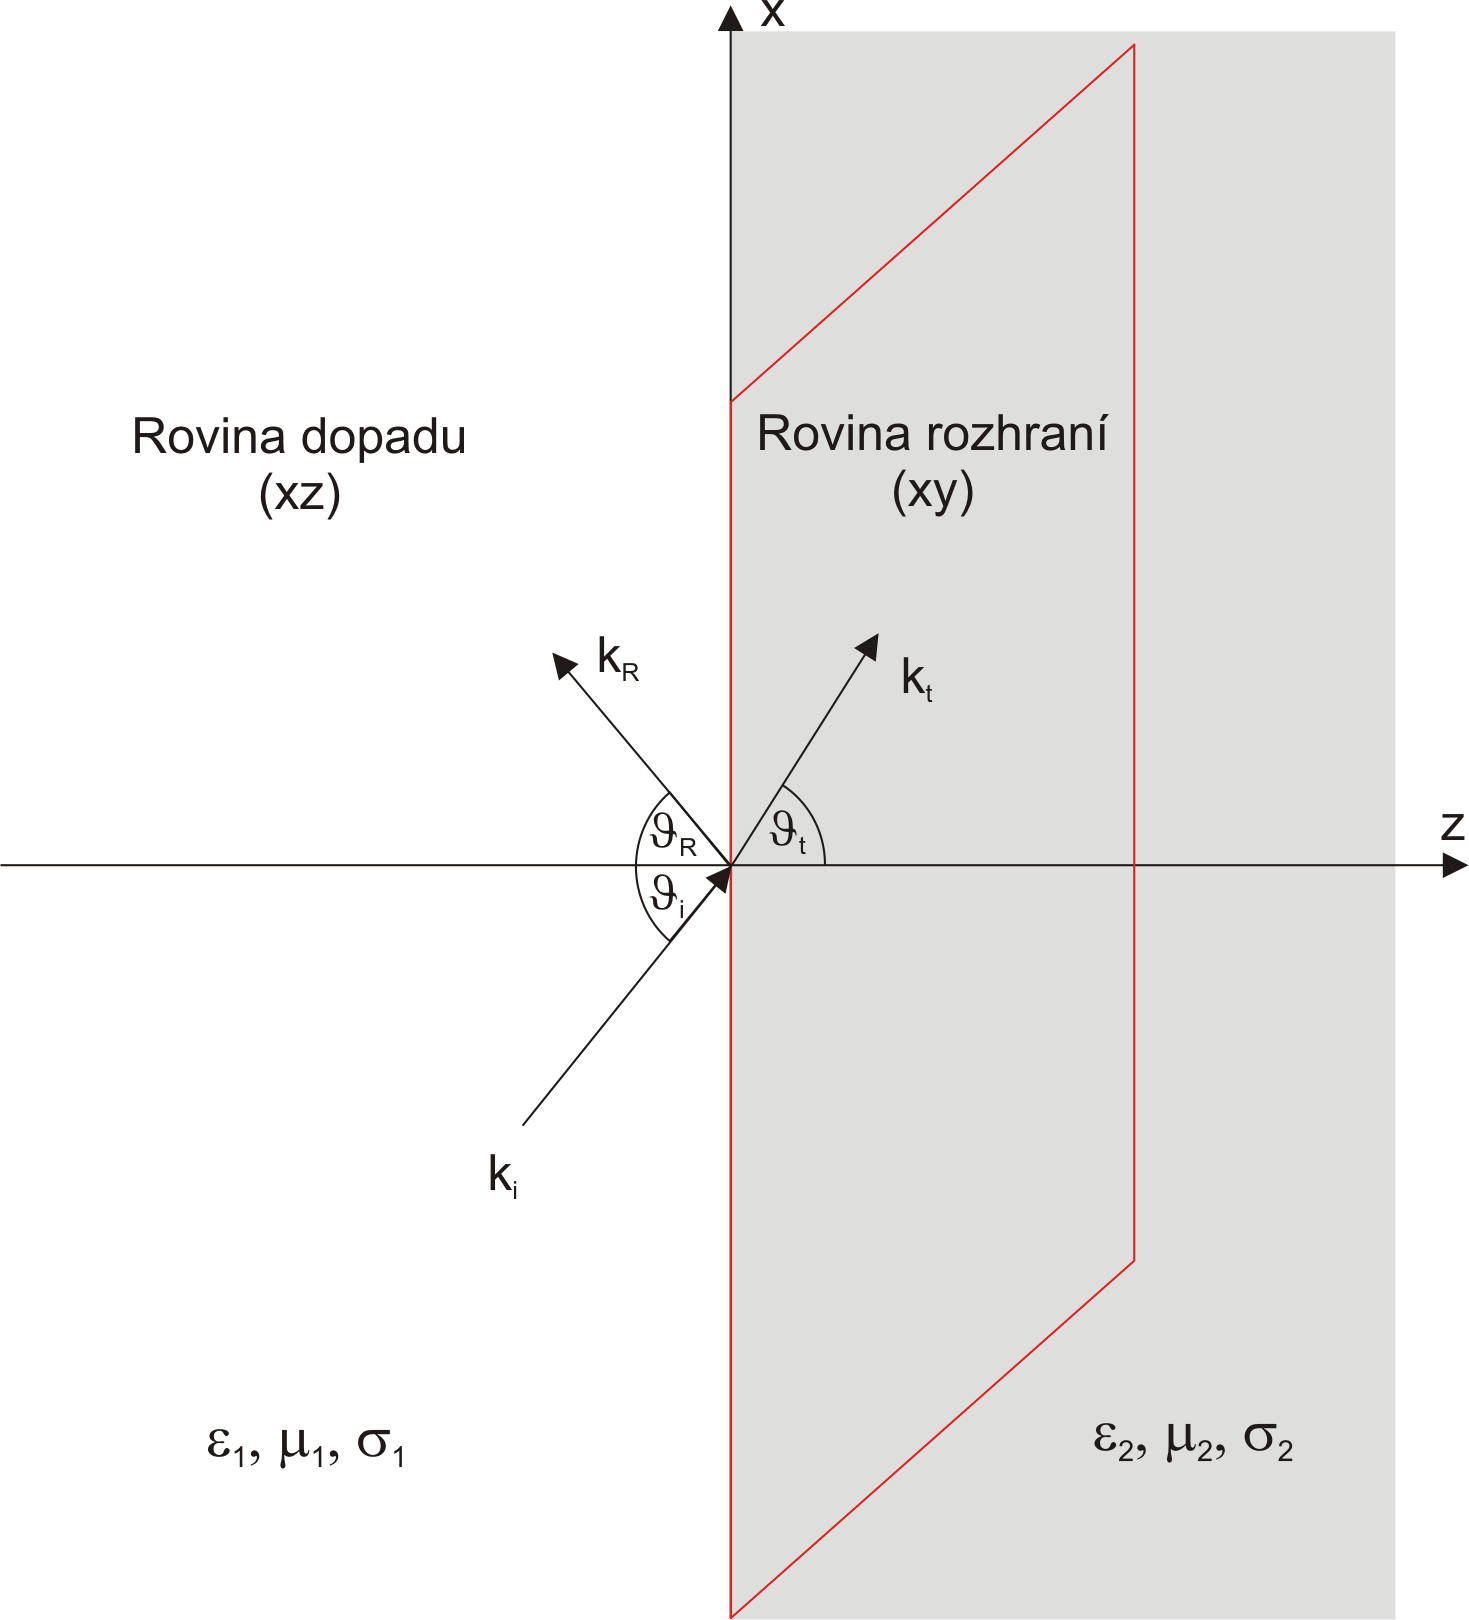
\includegraphics[width=10.5cm]{evlny_rovinne_rozhrani.png}
	\caption{Obecný dopad rovinné vlny na rozhraní.}
	\label{obr:evlny_rovinne_rozhrani}
\end{figure}

Jak je navíc z obrázku patrné, hranice mezi prostředími leží v rovině $xy$. Označuje se jako {\bf rovina rozhraní}. Jednotlivé prostředí se liší materiálovými konstantami $\varepsilon$, $\mu$ a $\sigma$. Vlna se šíří ve směru osy $z$, tak jak bylo uvažováno již v podkapitole \ref{sec:evlny_volne_prostredi}. Dopadá na rovinu rozhraní pod úhlem $\vartheta_{i}$ (z anglického \uv{incident wave}). Část vlny se odráží pod úhlem $\vartheta_{r}$ (\uv{ref{l}ected}) a část proniká pod úhlem $\vartheta_{t}$ (\uv{transmitted}). Vlnové vektory všech tří variant jsou vyznačeny na obrázku \ref{obr:evlny_rovinne_rozhrani}. Rovina, ve které leží vektor dopadající vlny $k_{i}$, tvořená osami $xz$, se značí jako {\bf rovina dopadu}.

Splnění podmínek na rozhraní pro tečné složky vektorů $\vec E$ a $\vec H$ nastane, když jsou shodné x-ové složky vlnových vektorů, tj. $k_{ix} = k_{rx} = k_{tx}$. Dle obrázku \ref{obr:evlny_rovinne_rozhrani} je patrné, že s využitím naznačených úhlů, lze zapsat.
\begin{displaymath}
	k_{i}sin\vartheta_{i} = k_{r}sin\vartheta_{r} = k_{t}sin\vartheta_{t}
\end{displaymath}
Vzhledem k shodnosti prostředí, ve kterém se nachází postupná a odražená vlna, je možné zavédst přiřazení $k_{1} = k_{i} = k_{r}$. Pro úplnost se ještě přeznačí $k_{2} = k_{t}$. Vyjádřený vztah (\ref{rce:evlny_snell_odvozeni}) je výchozím pro Snellovy zákony.
\begin{equation}
	k_{1}sin\vartheta_{i} = k_{1}sin\vartheta_{r} = k_{2}sin\vartheta_{t}
	\label{rce:evlny_snell_odvozeni}
\end{equation}
\begin{description}
\item[Zákon odrazu] Platí pro dopadající a odraženou vlnu. Lze jej také ústně interpretovat jako:\hspace{2cm} \uv{Úhel odrazu se rovná úhlu dopadu.}
\end{description}
\begin{displaymath}
	k_{1}sin\vartheta_{i} = k_{1}sin\vartheta_{r}
\end{displaymath}
\begin{equation}
	\vartheta_{i} = \vartheta_{r}
	\label{rce:evlny_zakon_odrazu}
\end{equation}
\begin{description}
\item[Zákon lomu] Platí opět pro dopadající vlnu a pro vlnu pronikající do druhého prostředí.
\end{description}
\begin{displaymath}
	k_{1}sin\vartheta_{i} = k_{2}sin\vartheta_{t}
\end{displaymath}
\begin{equation}
	\frac{k_{2}}{k_{1}} = \frac{sin\vartheta_{i}}{sin\vartheta_{t}}
	\label{rce:evlny_zakon_lomu}
\end{equation}

\subsection{Kolmý dopad rovinné vlny na rozhraní} \label{subsec:kolmy_dopad}
V konkrétním případě, dle obrázku \ref{obr:evlny_dielektricke_rozhrani}, je naznačen dopad rovinné homogenní vlny na rovinné rozhraní mezi dvěmi prostředími. Ty jsou popsány obecně materiálovými paramtery $\varepsilon_{1,2}$, $\mu_{1,2}$ a $\sigma_{1,2}$. Z nich je možné vztahem $Z=\sqrt{\frac{j\omega\mu}{j\omega\varepsilon + \sigma}}$ vyjádřit vlnové impedance pro jednotlivé prostředí.

\begin{figure}[!h]
	\centering
	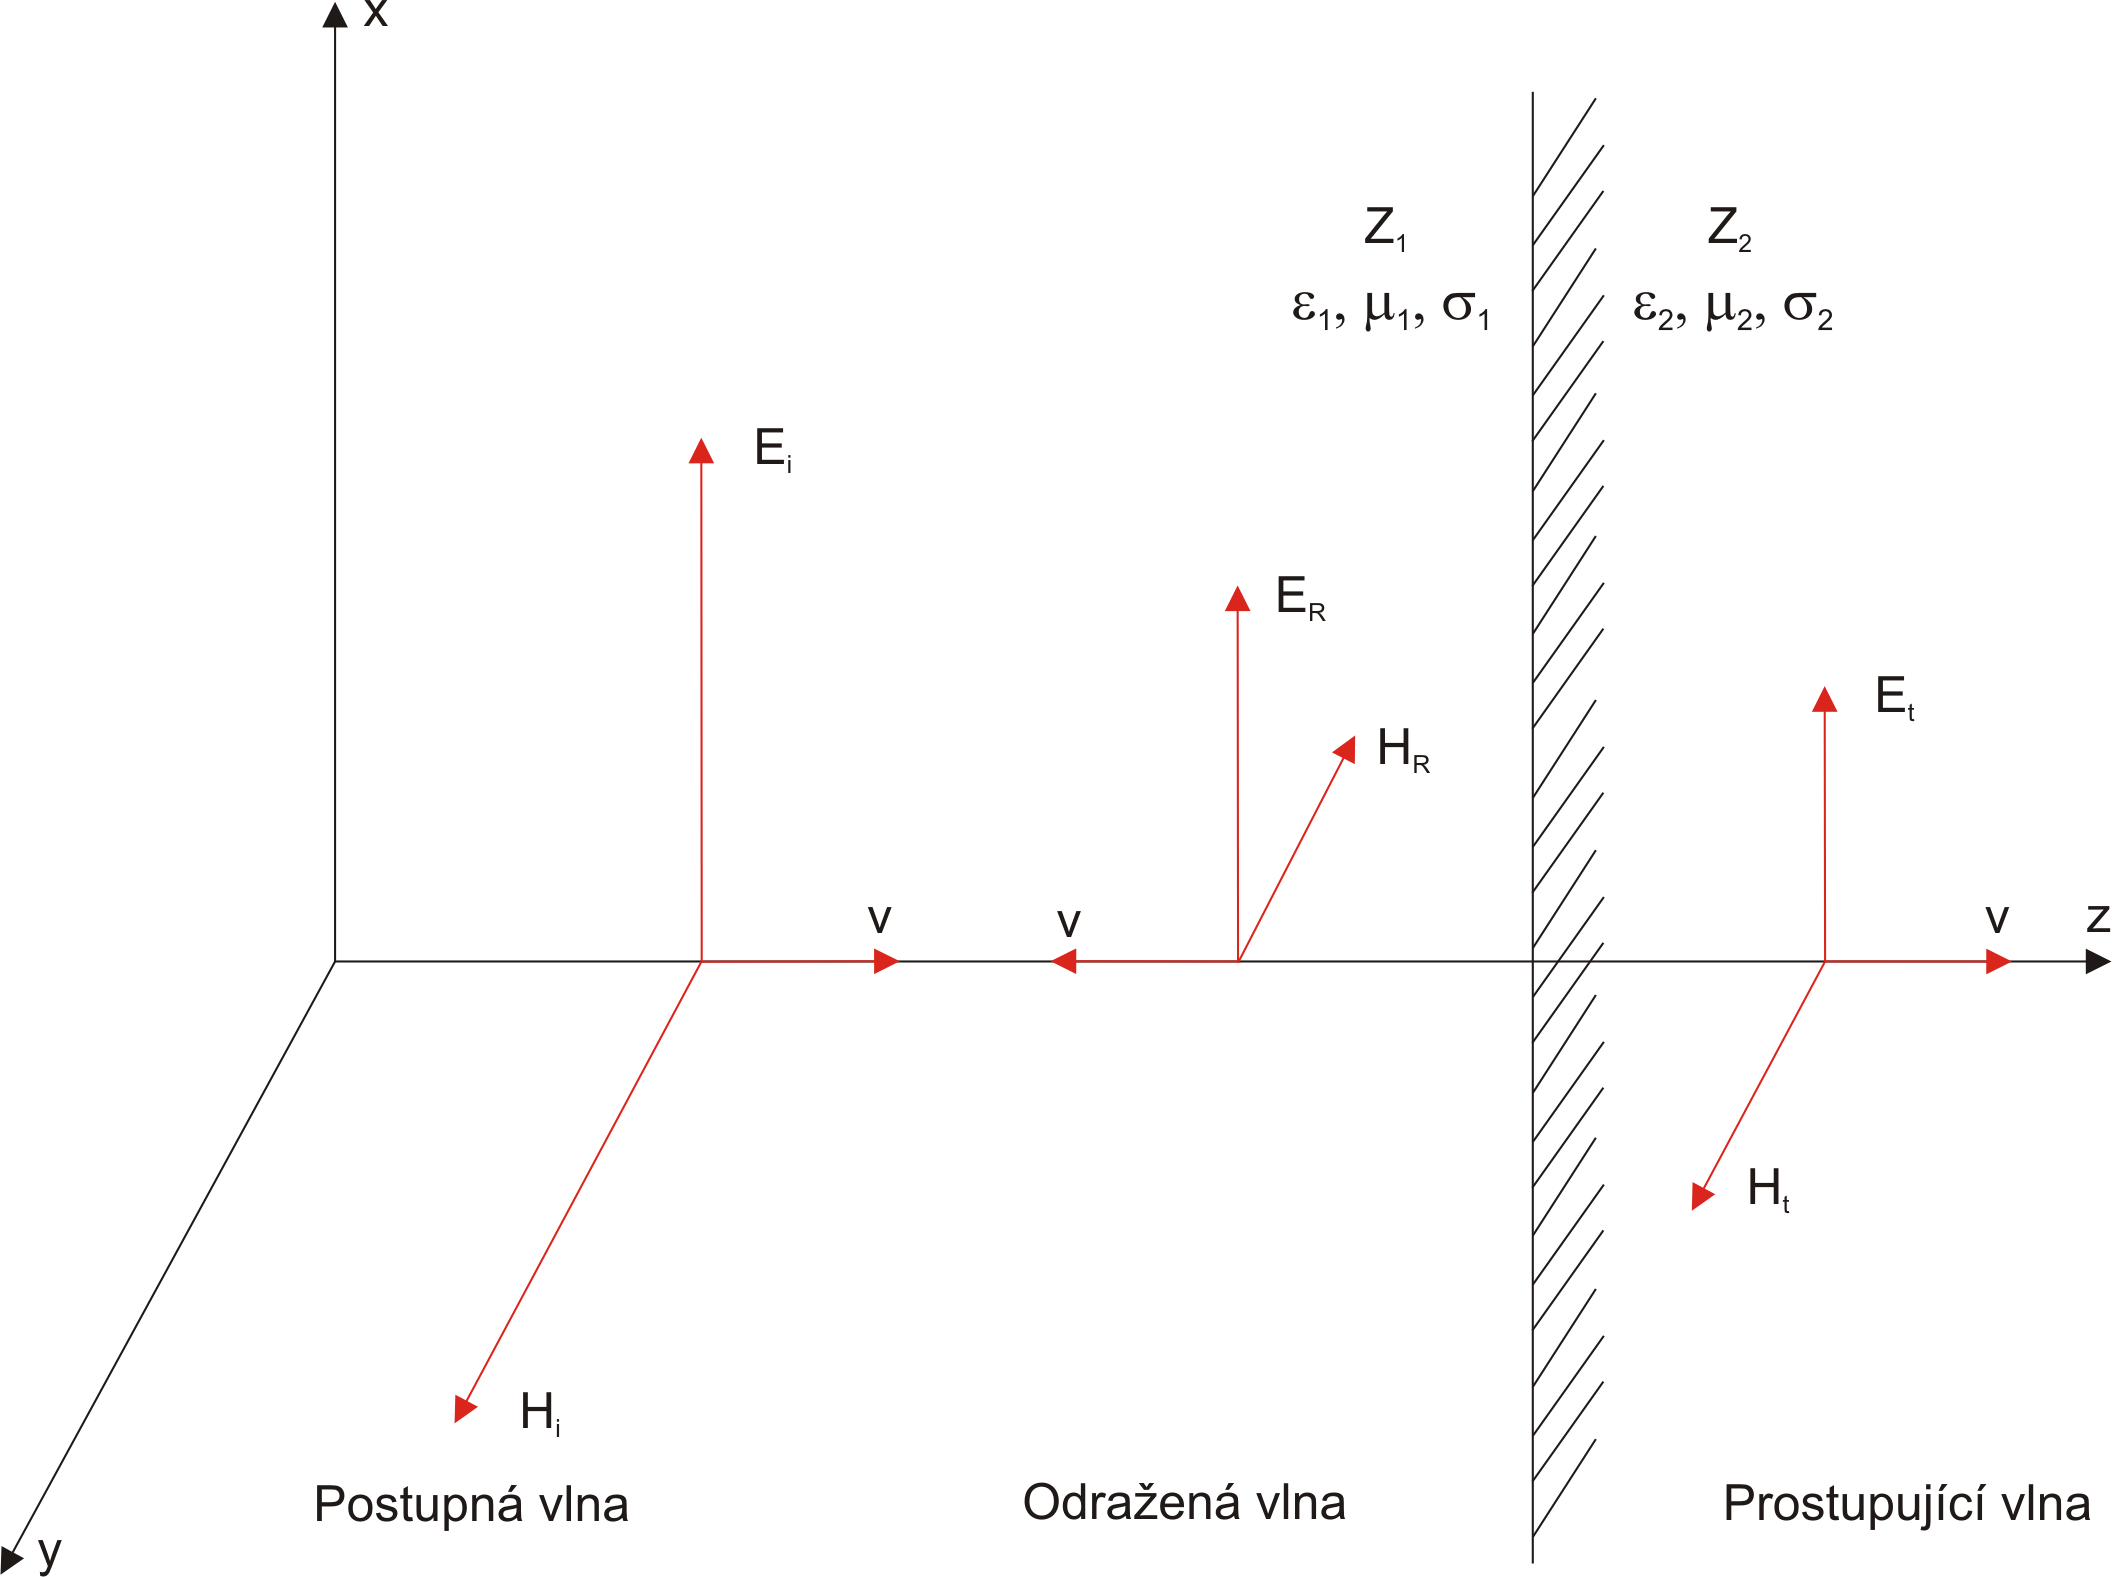
\includegraphics[width=13.5cm]{evlny_dielektricke_rozhrani.png}
	\caption{Kolmý dopad rovinné vlny rozhraní mezi dielektriky.}
	\label{obr:evlny_dielektricke_rozhrani}
\end{figure}

Vlna, která dopadá na rozhraní, lze zapsat vztahy pro vektory intezity elektrického pole $\vec E_{i}$ a magnetického $\vec H_{i}$ v závislosti na souřadnici $z$.
\begin{displaymath}
	\vec{E_{i}}(z) = E_{i0}e^{-jk_{1}z}\vec{x_{0}}
\end{displaymath}
\begin{displaymath}
	\vec{H_{i}}(z) = \frac{E_{i0}}{Z_{1}}e^{-jk_{1}z}\vec{y_{0}}
\end{displaymath}
Pro odraženou vlnu platí.
\begin{displaymath}
	\vec{E_{r}}(z) = E_{r0}e^{jk_{1}z}\vec{x_{0}}
\end{displaymath}
\begin{displaymath}
	\vec{H_{r}}(z) = - \frac{E_{r0}}{Z_{1}}e^{jk_{1}z}\vec{y_{0}}
\end{displaymath}
A nakonec pro prostupující vlnu.
\begin{displaymath}
	\vec{E_{t}}(z) = E_{t0}e^{-jk_{2}z}\vec{x_{0}}
\end{displaymath}
\begin{displaymath}
	\vec{H_{t}}(z) = \frac{E_{t0}}{Z_{2}}e^{-jk_{2}z}\vec{y_{0}}
\end{displaymath}
Podle podmínek na rozhraní ($z = 0$) se určí závislosti komplexních amplitud. Vychází se z~uvedených vztahů pro dopadající, odraženou a pronikající vlnu.
Pro vektor intenzity elektrického pole platí.
\begin{displaymath}
	\vec{E_{i}}(0) + \vec{E_{r}}(0)  = \vec{E_{t}}(0)
\end{displaymath}
\begin{displaymath}
	 E_{i0}e^{-jk_{1}0}\vec{x_{0}} + E_{r0}e^{jk_{1}0}\vec{x_{0}}  = E_{t0}e^{-jk_{2}0}\vec{x_{0}}
\end{displaymath}
\begin{equation}
	E_{i0} + E_{r0}  = E_{t0}
	\label{rce:evlny_rozhrani_E}
\end{equation}
Pro vektor intenzity magnetického pole na daném rozhraní se jedná o analogické odvození, tj. $\vec{H_{i}}(0) + \vec{H_{r}}(0)  = \vec{H_{t}}(0)$, čímž dostaneme.
\begin{equation}
	\frac{E_{i0}-E_{r0}}{Z_{1}} = \frac{E_{t0}}{Z_{2}}
	\label{rce:evlny_rozhrani_H}
\end{equation}
Za $E_{t0}$ se dosadí z rovnice (\ref{rce:evlny_rozhrani_E}) do (\ref{rce:evlny_rozhrani_H}) . Dostaneme závislost $E_{r0}$ na $E_{i0}$, na jejíž základě se dle \cite{emp} definuje {\bf činitel odrazu (reflexe)}  $R = \frac{E_{r0}}{E_{i0}}$. 
\begin{displaymath}
	\frac{E_{i0}-E_{r0}}{Z_{1}} = \frac{E_{i0} + E_{r0}}{Z_{2}}
\end{displaymath}
\begin{displaymath}
	E_{r0}\Big( \frac{1}{Z_{1}} + \frac{1}{Z_{2}} \Big) = E_{i0}\Big( \frac{1}{Z_{1}} - \frac{1}{Z_{2}} \Big)
\end{displaymath}
\begin{equation}
	E_{r0} = E_{i0} \frac{Z_{2}-Z_{1}}{Z_{1}+Z_{2}}
	\label{rce:evlny_cin_odrazu_odvozeni}
\end{equation}
Z rovnice (\ref{rce:evlny_cin_odrazu_odvozeni}) je patrný činitel odrazu.
\begin{equation}
	R = \frac{Z_{2}-Z_{1}}{Z_{1}+Z_{2}}
	\label{rce:evlny_cin_odrazu}
\end{equation}
 Pokud chceme vyjádřit závislost $E_{t0}$ na $E_{i0}$ dosadíme z (\ref{rce:evlny_rozhrani_E}) do (\ref{rce:evlny_rozhrani_H}) za $E_{r0}$. Následně se určuje {\bf činitel prostupu (transmise)}  $T = \frac{E_{t0}}{E_{i0}}$. 
\begin{displaymath}
	\frac{E_{i0}-E_{t0}+E_{i0}}{Z_{1}} = \frac{E_{t0}}{Z_{2}}
\end{displaymath}
\begin{displaymath}
	E_{t0} \frac{Z_{1}+Z_{2}}{Z_{1}Z_{2}} = E_{i0} \frac{2}{Z_{1}}
\end{displaymath}
\begin{equation}
	E_{t0} = E_{i0} \frac{2Z_{2}}{Z_{1}+Z_{2}}
	\label{rce:evlny_cin_prostupu_odvozeni}
\end{equation}
V (\ref{rce:evlny_cin_prostupu_odvozeni}) je opět zřejmý činitel prostupu.
\begin{equation}
	T = \frac{2Z_{2}}{Z_{1}+Z_{2}}
	\label{rce:evlny_cin_prostupu}
\end{equation}
Vztahy pro oba činitele (\ref{rce:evlny_cin_prostupu}) a (\ref{rce:evlny_cin_odrazu}) jsou na sobě závislé a řídí se vztahem $1 + R = T$.

\subsection{Dopad rovinné vlny pod obecným úhlem}
Při analýze chování dopadající rovinné vlny pod jiným úhlem, než aby se jednalo o kolmý dopad, se rozlišuje, zda se jedná o kolmou (horizontální) nebo rovnoběžnou (vertikální) polarizaci vlny. Orientace se určiuje podle vektoru intenzity elektrického pole $\vec E$.
\subsubsection*{Kolmá polarizace}
Vektor $\vec E$ je v tomto případě kolmý na rovinu dopadu, tj. $xz$, podle obrázku \ref{obr:evlny_kolma_polarizace}.

\begin{figure}[!h]
	\centering
	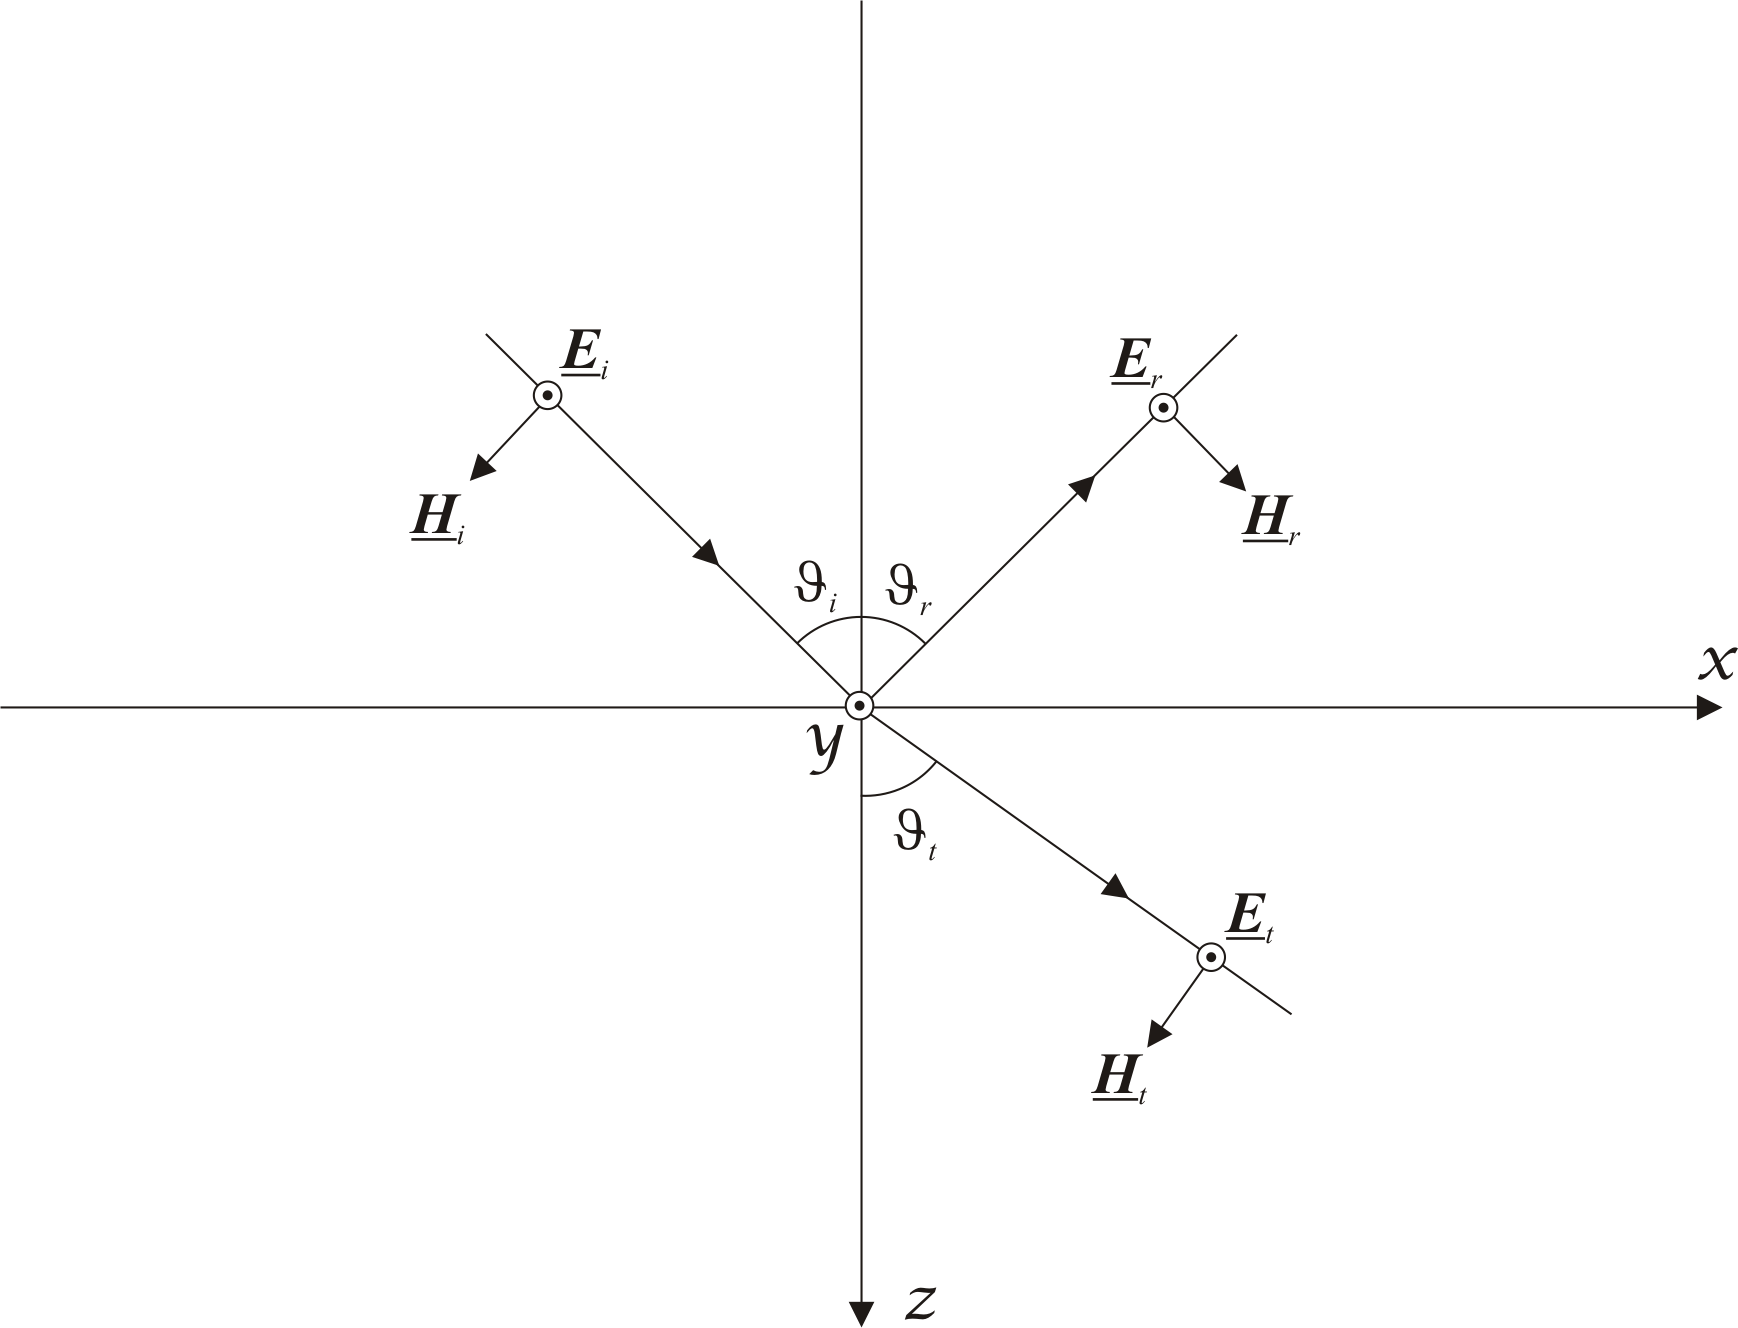
\includegraphics[width=10cm]{evlny_kolma_polarizace.png}
	\caption{Kolmá polarizace rovinné vlny.\cite{emp}}
	\label{obr:evlny_kolma_polarizace}
\end{figure}

Podobně jako v části \ref{subsec:kolmy_dopad} se také u této varianty uspořádání definují činitelé odrazu $R$ a prostupu $T$. Analogickým způsobem bychom dostali vztahy, které jsou blíže odvozené v \cite[str. 94]{emp} a pro které obdobně platí $R_{\perp} + 1 = T_{\perp}$.
\begin{equation}
	R_{\perp} = \frac{E_{r0}}{E_{i0}} = \frac{Z_{2}cos\vartheta_{i}-Z_{1}cos\vartheta_{t}}{Z_{2}cos\vartheta_{i}+Z_{1}cos\vartheta_{t}} = \frac{Z_{2}cos\vartheta_{i}-Z_{1}\sqrt{1-(k_{1}/k_{2})^{2}sin^{2}\vartheta_{i}}}{Z_{2}cos\vartheta_{i}+Z_{1}\sqrt{1-(k_{1}/k_{2})^{2}sin^{2}\vartheta_{i}}}
	\label{rce:evlny_cin_odrazu_kolma}
\end{equation}
\begin{equation}
	T_{\perp} = \frac{E_{t0}}{E_{i0}} = \frac{2Z_{2}cos\vartheta_{i}}{Z_{2}cos\vartheta_{i}+Z_{1}cos\vartheta_{t}} = \frac{2Z_{2}cos\vartheta_{i}}{Z_{2}cos\vartheta_{i}+Z_{1}\sqrt{1-(k_{1}/k_{2})^{2}sin^{2}\vartheta_{i}}}
	\label{rce:evlny_cin_prostupu_kolma}
\end{equation}

\subsubsection*{Rovnoběžná polarizace}
Pro vektor intenzity elektrického pole platí, že je tentokrát rovnoběžný s rovinou dopadu $xz$. Současně je vektror $\vec H$ tečný k rovině rozhraní $xy$, viz. obrázek \ref{obr:evlny_rovnobezna_polarizace}.

\begin{figure}[!h]
	\centering
	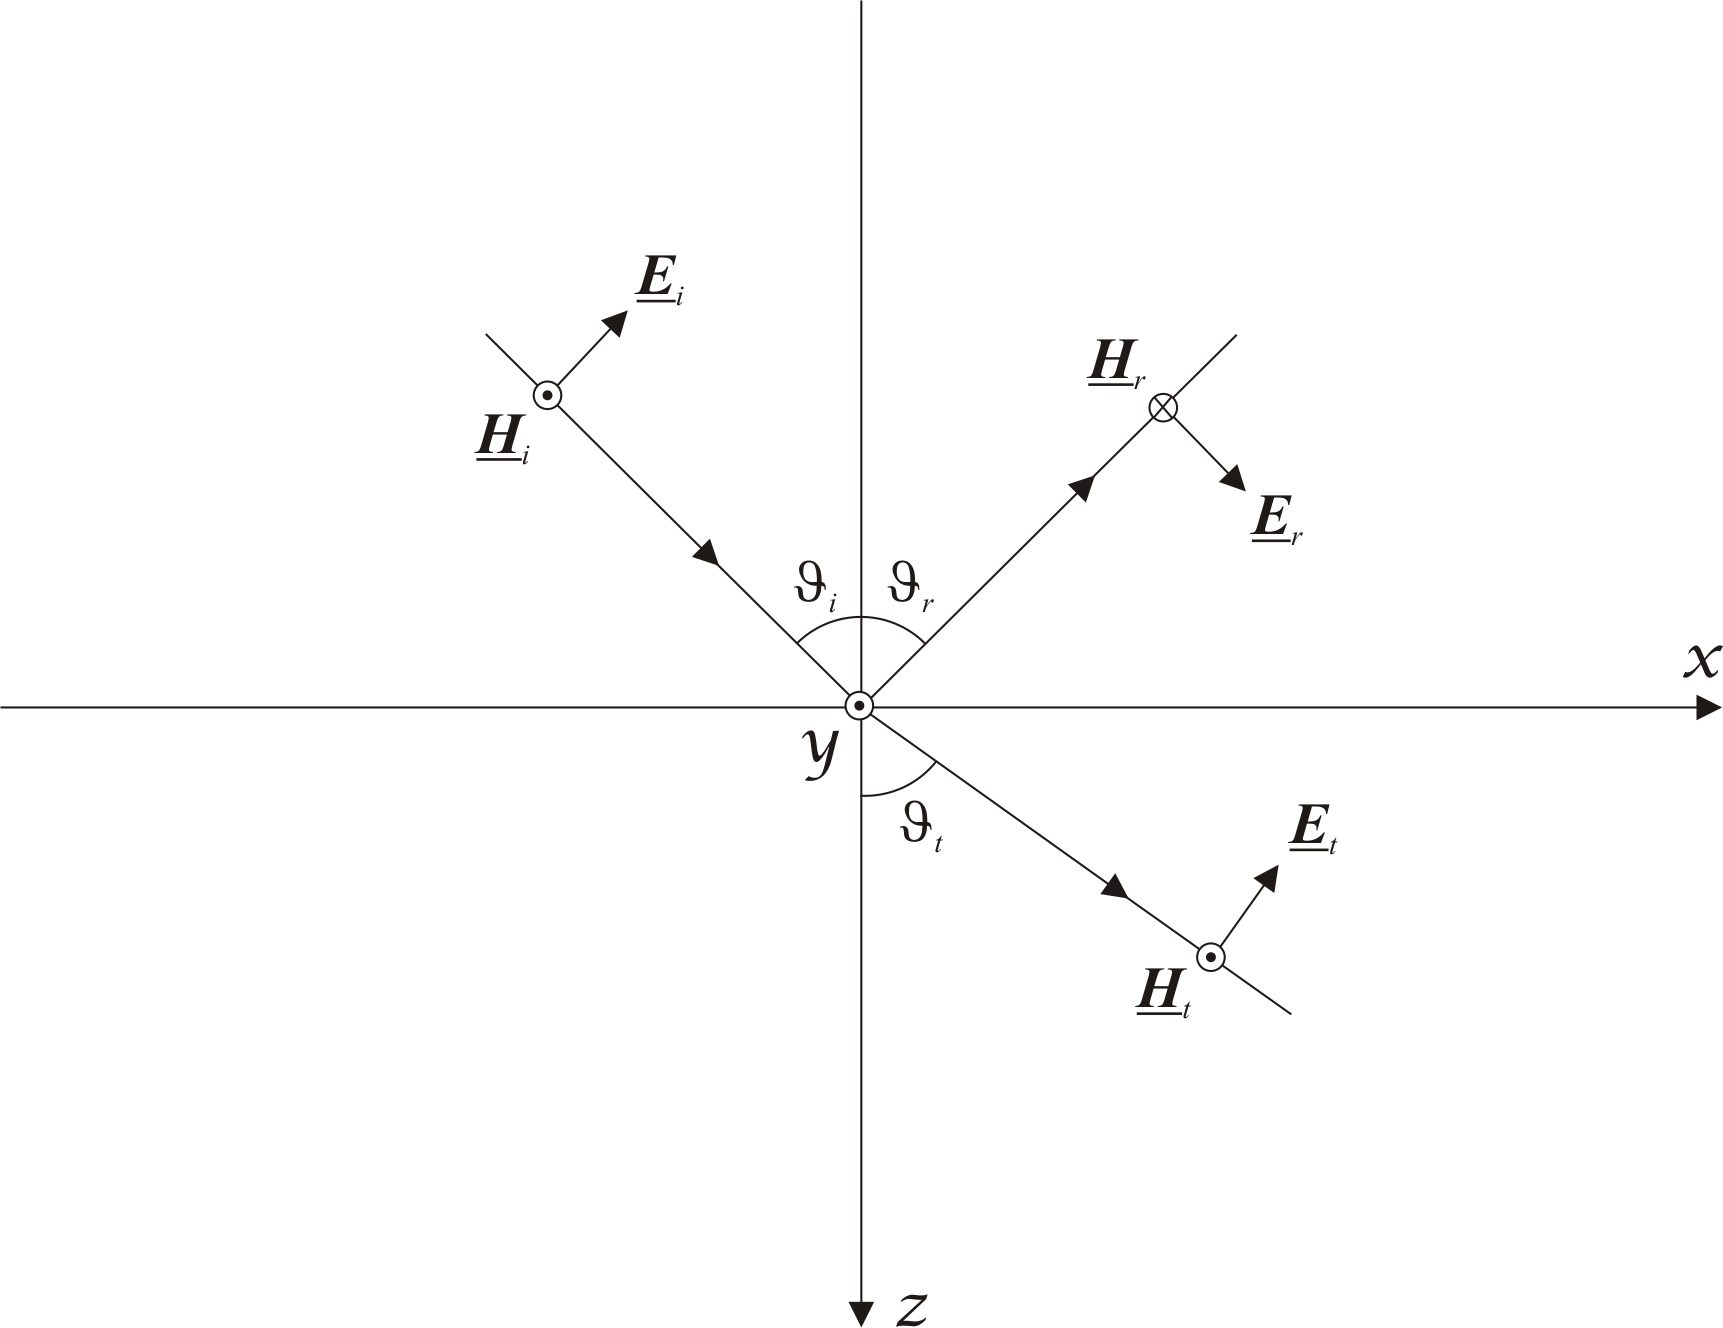
\includegraphics[width=10cm]{evlny_rovnobezna_polarizace.png}
	\caption{Rovnoběžná polarizace rovinné vlny.\cite{emp}}
	\label{obr:evlny_rovnobezna_polarizace}
\end{figure}

Odvození vztahů pro činitele odrazu a prostupu se nachází v \cite[str. 95]{emp}. Pro výsledné vztahy platí v tomto případě $R_{\parallel} + 1 = T_{\parallel}\frac{cos\vartheta_{t}}{cos\vartheta_{i}}$.
\begin{equation}
	R_{\parallel} = \frac{E_{r0}}{E_{i0}} = \frac{Z_{2}cos\vartheta_{t}-Z_{1}cos\vartheta_{i}}{Z_{2}cos\vartheta_{t}+Z_{1}cos\vartheta_{i}} = \frac{Z_{2}\sqrt{1-(k_{1}/k_{2})^{2}sin^{2}\vartheta_{i}}-Z_{1}cos\vartheta_{i}}{Z_{2}\sqrt{1-(k_{1}/k_{2})^{2}sin^{2}\vartheta_{i}}+Z_{1}cos\vartheta_{i}}
	\label{rce:evlny_cin_odrazu_rovnobezna}
\end{equation}
\begin{equation}
	T_{\parallel} = \frac{E_{t0}}{E_{i0}} = \frac{2Z_{2}cos\vartheta_{i}}{Z_{2}cos\vartheta_{t}+Z_{1}cos\vartheta_{i}} = \frac{2Z_{2}cos\vartheta_{i}}{Z_{2}\sqrt{1-(k_{1}/k_{2})^{2}sin^{2}\vartheta_{i}}+Z_{1}cos\vartheta_{i}}
	\label{rce:evlny_cin_prostupu_rovnobezna}
\end{equation}
Vztahy (\ref{rce:evlny_cin_odrazu_kolma}) až (\ref{rce:evlny_cin_prostupu_rovnobezna}) se také nazývají {\bf Fresnelovy rovnice}.

\subsection{Brewsterův polarizační úhel}
\subsubsection*{Situace u kolmé polarizace dopadající vlny}
Úhel $\vartheta_{i}$ se označuje jako Brewsterův polarizační při splnění určitých podmínek. Pokud obecně polarizovaná elektromagnetická vlna dopadne na rozhraní pod tímto úhlem, tak odražená vlna bude mít pouze složku rovnoběžnou s rovinou dopadu $xz$.

Odvození vychází ze vztahu pro $R_{\perp}$ (\ref{rce:evlny_cin_odrazu_kolma}). Pokud bude platit $Z_{2}cos\vartheta_{i} = Z_{1}cos\vartheta_{t}$, tak činitel odrazu $R_{\perp}$ vyjde nulový. To mimo jiné znamená, že se kolmo polarizovaná vlna neodráží a úplně celá prostupuje do druhého prostředí. Pomocí zákona lomu (\ref{rce:evlny_zakon_lomu}) a~vztahu $cos\vartheta_{t} = \sqrt{1-sin^{2}\vartheta_{t}}$ dostaneme.
\begin{equation}
	Z_{2}cos\vartheta_{i} = Z_{1}\sqrt{1-\bigg(\frac{k_{1}}{k_{2}}\bigg)^{2}sin^{2}\vartheta_{i}}
	\label{rce:evlny_brewster_kolma_odvozeni}
\end{equation}
Tento vztah (\ref{rce:evlny_brewster_kolma_odvozeni}) má řešení pro prostředí, kde platí $\mu_{1} \ne \mu_{2}$ a zároveň $\varepsilon_{1} = \varepsilon_{2}$. Výsledný výraz pro {\bf Brewsterův polarizační úhel} platí tedy pro tuto závislost materiálových konstant.
\begin{equation}
	sin\vartheta_{i\ BR} = \frac{1}{\sqrt{1+\frac{\mu_{1}}{\mu_{2}}}}
	\label{rce:evlny_brewster_kolma}
\end{equation}

\subsubsection*{Rovnoběžná polarizace dopadající vlny}
Analogickým postupem jako v předchozím případě vycházíme ze vztahu (\ref{rce:evlny_cin_odrazu_rovnobezna}) pro $R_{\parallel}$. Zde se pro $Z_{2}cos\vartheta_{t} = Z_{1}cos\vartheta_{i}$ neodráží rovnoběžně polarizovaná vlna. Vztah Brewsterova polarizačního úhlu platí pro dielektrika ($\varepsilon_{1} \ne \varepsilon_{2}$), kde se po dopadu obecně polarizované vlny odráží složka polarizovaná kolmo na rovinu dopadu $xz$.
\begin{equation}
	sin\vartheta_{i\ BR} = \frac{1}{\sqrt{1+\frac{\varepsilon_{1}}{\varepsilon_{2}}}}
	\label{rce:evlny_brewster_kolma}
\end{equation}
\newpage

\section{Vrstvené prostředí}

\begin{equation}
	\vec{E_{R}} + \vec{E_{TRT}} + \vec{E_{TRRRT}} + \ldots
	\label{rce:evlny_vrstvene_rada}
\end{equation}


\subsection{Metody řešení vln ve vrstveném prostředí}
Řešení chování elektromagnetické vlny na tomto typu rozhraní vychází z vyčíslení řady (\ref{rce:evlny_vrstvene_rada}). To je samo o sobě ve většině případů velmi komplikované. Jednotlivé členy je pak potřeba sečíst s ohledem na amplitudu a fázi. Pro řešení však existuje několik zjednodušujících metod.
\begin{enumerate}
\item Součet vln stejného směru a vyjádření jedinou vlnou.
\item Maticová metoda.
\item Princip založený na analýze vedení.
\end{enumerate}
\newpage

\section{Vlnovody}
\subsection{Klasifikace vln}
str.112 - TEM, TE, TM, HE, EH\\
str.108 - obecně\\
str.131 - TE, Ez = 0, TM Hz = 0\\
str.143 - Snell\\
\subsection{Kritická frekvence}
str.132
\newpage

\section{Dutinové rezonátory}
str.150\\
str.151 - rez. kmitočet\\
\newpage